\documentclass{article}


\usepackage{arxiv}

\usepackage[utf8]{inputenc} % allow utf-8 input
\usepackage[T1]{fontenc}    % use 8-bit T1 fonts
\usepackage{hyperref}       % hyperlinks
\usepackage{url}            % simple URL typesetting
\usepackage{booktabs}       % professional-quality tables
\usepackage{array}          % extended tabular column formatting
\usepackage{amsfonts}       % blackboard math symbols
\usepackage{nicefrac}       % compact symbols for 1/2, etc.
\usepackage{microtype}      % microtypography
\usepackage{graphicx}
\graphicspath{{figures/}{./}}
\usepackage{subcaption}
\usepackage{float}
\usepackage{amsmath}
\usepackage{amsthm}         % for theorems, lemmas etc
\usepackage[numbers]{natbib}
\usepackage{doi}
\usepackage{enumitem}

\theoremstyle{plain}
\newtheorem{theorem}{Theorem}[section]
\newtheorem{proposition}[theorem]{Proposition}
\newtheorem{lemma}[theorem]{Lemma}
\newtheorem{corollary}[theorem]{Corollary}
\newtheorem{fact}[theorem]{Fact}

\theoremstyle{definition}
\newtheorem{definition}[theorem]{Definition}
\newtheorem{example}[theorem]{Example}
\newtheorem{remark}[theorem]{Remark}
\newtheorem{remarks}[theorem]{Remarks}

\newcommand{\Cov}{\mathrm{Cov}}
\newcommand{\Var}{\mathrm{Var}}

\title{The HP Protein-Folding Problem: Modern Constraint Programming and Reinforcement Learning approaches}

\author{
    \href{https://orcid.org/0009-0000-0270-7112}{
\includegraphics[scale=0.06]{orcid.pdf}\hspace{1mm}Pranav Ramanathan} \\
    School of Mathematical Sciences\\
    Queen Mary University of London\\
    \texttt{p.ramanathan@se23.qmul.ac.uk}
    \And%
    \href{https://orcid.org/0000-0003-0519-6762}{
\includegraphics[scale=0.06]{orcid.pdf}\hspace{1mm}Thomas Prellberg} \\
    School of Mathematical Sciences\\
    Queen Mary University of London\\
    \texttt{t.prellberg@qmul.ac.uk}
}

%%% Add PDF metadata to help others organize their library
\hypersetup{
    pdftitle={The HP Protein-Folding Problem: Comparing Constraint Programming and Reinforcement Learning},
    pdfsubject={cs.AI,q-bio.BM},
    pdfauthor={Pranav Ramanathan, Thomas Prellberg},
    pdfkeywords={HP model, protein folding, constraint programming, CP-SAT, reinforcement learning, deep Q-learning, lattice models}
}

\begin{document}
\raggedbottom%
\maketitle

\begin{abstract}

This paper presents a modern approach to constraint programming for the HP protein folding problem using Google OR-Tools CP-SAT, and compares it with Reinforcement Learning (RL). The HP model is designed to model a protein as a sequence of H (hydrophobic) and P (polar) amino acids on a simple cubic lattice with the interactions being chosen to mimic an aqueus solvent. Minimising its energy is a classic NP-complete problem in computational physics and combinatorial optimization, that has been studied extensively. CP-SAT is an open-source constraint programming solver that systematically explores the solution space through constraint satisfaction, dynamically augmenting itself with learned clauses. RL folds proteins by interacting with the environment and optimizing a policy through trial-and-error. On the shorter benchmark sequences tested, CP-SAT matches the best-known energy levels and provides certificates of optimality where it terminates with \texttt{OPTIMAL} status; on the longer sequences both methods remain below the best-known energies under the tested budgets.

% The Deep Q-Learning approach, including the Q-network architecture, experience replay, and reward structure for maximizing H-H contacts, is also discussed.

% This paper discusses the main components of the CP-SAT approach, such as constraint formulation, contact maximization, and symmetry breaking, and explains how it is used to solve the HP protein-folding problem. 
\end{abstract}

\keywords{HP model \and protein folding \and constraint programming \and CP-SAT \and reinforcement learning \and lattice models}

\section{Introduction}

% Proteins are biological macromolecules that fold into three-dimensional structures, which determine their unique functions. These functions range from catalysing biochemical reactions to defending against pathogens. Because a protein's activity is strongly shaped by its conformation, characterising folding behaviour is often essential for understanding how proteins interact with other molecules. In medicine, this can inform drug discovery by supporting the design of compounds intended to stabilise or otherwise modulate specific protein structures.

% This brings us to a central challenge in molecular biology: predicting a protein's three-dimensional conformation from its amino acid sequence. That task matters for drug design, disease research, and protein engineering. Levinthal's Paradox, introduced by Cyrus Levinthal in 1969~\cite{Levinthal1969}, is often cited to show why an exhaustive search over all possible conformations is not a realistic explanation for how proteins fold. The key observation is that, even under conservative assumptions, the conformational search space becomes astronomically large.

% Haemoglobin provides a useful illustration. The oxygen-carrying protein in red blood cells has a beta subunit containing 146 amino acids~\cite{NCBI_Hemoglobin}, and each position in the chain is drawn from 20 standard amino acid types~\cite{NCBI_AminoAcids}. What makes folding difficult is how quickly the space of plausible conformations expands as the chain grows. If each rotatable bond is assumed to have $k$ stable conformations and $n$ is the number of amino acids, a rough upper-bound count gives on the order of $k^{n-1}$ possible configurations. For a beta subunit that gives 145 rotatable bonds, taking $k$ as roughly 3 yields $3^{145}$, or about $10^{69}$ configurations. Even at an unrealistically fast sampling rate of one configuration per picosecond, enumerating the full set would take on the order of $10^{49}$ years. Yet haemoglobin folds spontaneously on millisecond-to-second timescales~\cite{Eaton1996}. The gap between these numbers is the intuition behind Levinthal's Paradox, and it is one reason folding is typically approached through models and algorithms that exploit structure rather than brute-force enumeration.
% design sequences
% other methods

Dill introduced the Hydrophobic-Polar (HP) lattice model in 1985~\cite{Dill1985}. This model collapses the twenty amino acid types into two classes: hydrophobic residues (H), which tend to avoid water, and polar residues (P), which interact more favourably with it. A sequence is then embedded as a self-avoiding walk on a lattice, with each residue occupying a distinct site and successive residues constrained to lie on adjacent lattice points~\cite{Lau1989}. Within this discrete setting, the objective is driven by hydrophobic contacts. In the simpler version of the model, the energy is defined by the number of non-consecutive H-H contacts, i.e., pairs of hydrophobic residues that are neighbours on the lattice but not adjacent along the chain. In effect, the optimisation target is to find an embedding that promotes hydrophobic clustering while respecting the self-avoidance and adjacency constraints.

Even under this simplified lattice formulation, HP folding remains computationally demanding. \textit{Crescenzi et al.}\ proved in 1998 that the optimisation problem is NP-complete~\cite{Crescenzi1998}, so one should not expect a method that scales efficiently across all instances as the sequence length increases. The practical consequences show up fairly quickly: by the time sequences are in the 30 to 50 residue range, the set of valid self-avoiding conformations is already large enough that exhaustive enumeration stops being a useful point of comparison. That is part of the reason the HP model is used so often in combinatorial optimisation research: it is clean to specify, hard to solve, and easy to evaluate consistently across algorithms.

Given that hardness, much of the earlier computational literature relied on heuristics rather than exact optimisation. Simulated annealing became a common choice from the 1990s onward because it provides a straightforward mechanism for escaping local minima by occasionally accepting unfavourable moves early in the search~\cite{UngerMoult1993}. Genetic algorithms offered a different style of exploration, maintaining a population of candidate folds and gradually improving it through recombination and mutation operators~\cite{Krasnogor2002Multimeme}. Tabu search was also explored, discouraging cycling by remembering recent states. Ant colony optimisation took yet another approach, biasing construction using information carried over from successful searches~\cite{LeshPullMoves2003, StützleACO2005}.

Constraint programming (CP) offers an alternative to heuristic search for HP folding. Chain connectivity, self-avoidance, and contact formation can all be encoded directly as folding constraints and then pruned through propagation~\cite{Barták2003}. Earlier CP tools, such as CPSP-tools, successfully tackled HP folding using specialised H-core databases and constraint satisfaction techniques~\cite{CPSP2009}. Google OR-Tools CP-SAT extends this approach by combining it with on-the-fly SAT-style clause learning and linear programming relaxation~\cite{Perron2023}. This can provide bounds on solution quality and, in favourable cases, certificates of optimality~\cite{GoogleORTools}. Large Neighbourhood Search is also supported, allowing solutions to be improved iteratively~\cite{Shaw1998}. Earlier domain-specific tools such as CPSP-tools~\cite{CPSP2009} solve HP folding by enumerating a precomputed database of optimal H-cores (connected lattice subgraphs of hydrophobic residues), then asking a constraint solver only whether the remaining polar residues can be threaded around each candidate core; this offline precomputation cannot be reused across lattice types or model variants. Our CP-SAT formulation instead encodes the full folding problem directly, trading some HP-specific power for portability, reproducibility, and direct comparability against a learning-based baseline on the same benchmark family.

While constraint programming guarantees optimality when feasible, its exponential scaling limits practical applicability to shorter sequences. Reinforcement learning has recently emerged as an alternative approach for HP folding. An attention-based deep Q-learning approach has recently been applied to the three-dimensional HP model~\cite{AttnDRL2504}. Folding was treated as a sequential decision problem, where agents can learn folding strategies through trial-and-error without explicitly encoding the problem constraints~\cite{Yang2022}. Whether this reinforcement learning method can compete with exact solver approaches like CP-SAT remains unknown.

This paper presents a modern approach to constraint programming for the 3D HP protein folding problem using Google OR-Tools CP-SAT, comparing it against the recent attention-based deep Q-learning method of~\cite{AttnDRL2504}. To enable a like-for-like comparison, we additionally rerun the RL baseline on hardware comparable to its published evaluation, so that both methods are exercised under the same operating conditions. Section~2 describes the implementation and training procedures for each method. Section~3 presents comparative results and scaling behaviour. Section~4 discusses algorithmic trade-offs, failure modes, and future research directions.

\section{Methodology}

\subsection{Problem Formulation}

The HP protein folding problem on a three-dimensional lattice is defined as follows. A protein sequence is represented as a string:
\begin{equation}
S = s_1 s_2 \ldots s_n,
\end{equation}
where each residue $s_i$ is classified as either hydrophobic (H) or polar (P). A conformation $C$ is a self-avoiding walk on the three-dimensional integer lattice $\mathbb{Z}^3$, meaning each residue is placed at a distinct position:
\begin{equation}
c_i = (x_i, y_i, z_i) \in \mathbb{Z}^3,
\end{equation}
and no two residues occupy the same lattice point. The adjacency constraint requires that consecutive residues along the chain are placed at Manhattan distance 1:
\begin{equation}
||c_i - c_{i+1}||_1 = 1 \quad \forall i \in \{1, \ldots, n-1\}.
\end{equation}
where $||v||_1 = |x| + |y| + |z|$ for a vector $v = (x, y, z)$.

The energy of a conformation is determined by the number of non-consecutive H-H contacts. A contact occurs when two hydrophobic residues are neighbours on the lattice but not adjacent along the sequence. Formally, the energy function is defined as
\begin{equation}
E(C) = -\left|\{(i,j) : s_i = s_j = \text{H}, \, |i - j| > 1, \, ||c_i - c_j||_1 = 1\}\right|,
\end{equation}
where the set counts all pairs of non-consecutive H-residues that are lattice-adjacent. The objective is to minimise $E(C)$, which is equivalent to maximising the number of favourable hydrophobic contacts. This formulation reflects the simplified physical principle that hydrophobic residues prefer to cluster together, shielding themselves from the surrounding aqueous environment. An illustration of this energy function is provided in Figure~\ref{fig:hp_lattice}.

\begin{figure}[H]
    \centering
    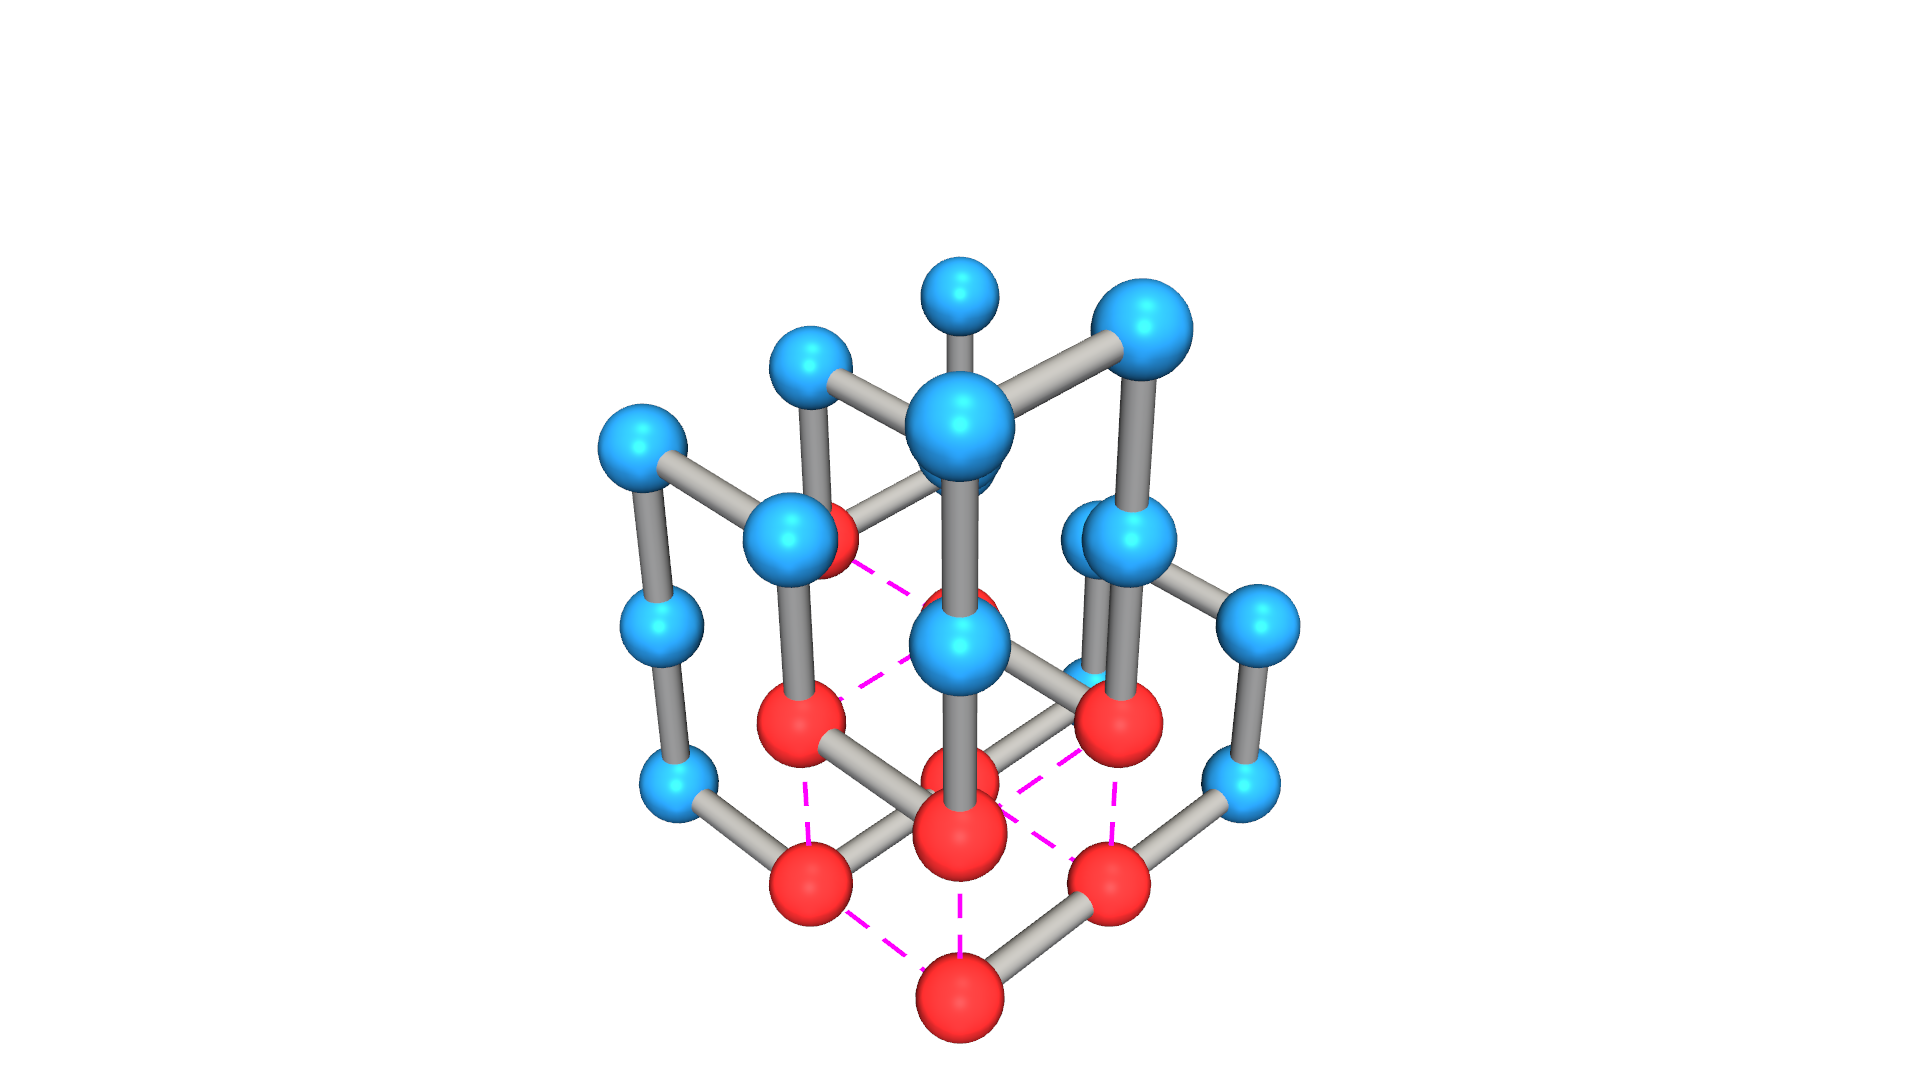
\includegraphics[width=0.6\textwidth]{3d3.png}
    \caption{Illustration of the 3D HP lattice model showing a short self-avoiding walk. Hydrophobic residues (H) are shown in red, polar residues (P) in blue. Dotted magenta lines indicate valid non-consecutive H-H contacts that contribute to the energy function; this conformation has energy $-9\epsilon_{HH}$.}\label{fig:hp_lattice}
\end{figure}

We evaluate both methods on a set of benchmark sequences drawn from the literature. Table~\ref{tab:benchmarks} lists the sequences used in this study, identified by their standard names (e.g., 3d1, 3d2, \ldots, 3d8). The sequences span a range of lengths from $n = 20$ to $n = 58$ residues and include both their H/P patterns and best-known energy values from prior work~\cite{AttnDRL2504}.

\begin{table}[htbp]
\centering
\caption{Benchmark HP sequences used in this study. Best-known energies are taken from~\cite{AttnDRL2504}.}\label{tab:benchmarks}
\begin{tabular}{lc>{\centering\arraybackslash}p{6.8cm}c}
\toprule
\textbf{Seq.} & \textbf{Length} & \textbf{Sequence} & \textbf{Best-known Energy} \\
\midrule
3d1 & 20 & ${(HP)}^{2}PH{(HP)}^{2}{(PH)}^{2}HP{(PH)}^{2}$ & $-11$ \\
3d2 & 24 & $H^{2}P^{2}{(HP^{2})}^{6}H^{2}$ & $-13$ \\
3d3 & 25 & $P^{2}HP^{2}{(H^{2}P^{4})}^{3}H^{2}$ & $-9$ \\
3d4 & 36 & $P{(P^{2}H^{2})}^{2}P^{5}H^{5}{(H^{2}P^{2})}^{2}P^{2}H{(HP^{2})}^{2}$ & $-18$ \\
3d5 & 46 & $P^2H^3PH^3P^3HPH^2PH^2P^2HPH^4$ \newline $PHP^2H^5PHPH^2P^2H^2P$ & $-35$ \\
3d6 & 48 & $P^{2}H{(P^{2}H^{2})}^{2}P^{5}H^{10}P^{6}$ \newline ${(H^{2}P^{2})}^{2}HP^{2}H^{5}$ & $-31$ \\
3d7 & 50 & $H^{2}{(PH)}^{3}PH^{4}PH{(P^{3}H)}^{2}P^{4}$ \newline ${(HP^{3})}^{2}HPH^{4}{(PH)}^{3}PH^{2}$ & $-34$ \\
3d8 & 58 & $PH{(PH^{3})}^{2}P{(PH^{2}PH)}^{2}H{(HP)}^{3}$ \newline ${(H^{2}P^{2}H)}^{2}PHP^{4}{(H{(P^{2}H)}^{2})}^{2}$ & $-44$ \\
\bottomrule
\end{tabular}
\end{table}


\subsection{CP-SAT Approach}\label{sec:cpsat_approach}

This section describes our constraint programming implementation using Google OR-Tools CP-SAT solver~\cite{GoogleORTools, Perron2023}. We formulate the 3D HP folding problem as a constraint satisfaction problem, encoding the self-avoiding walk and contact constraints algebraically to maximise H-H contacts.

\subsubsection{Decision Variables}

Our CP-SAT formulation uses one-hot encoding to represent where residues sit on the 3D cubic lattice. In one-hot encoding, each position is indicated by a binary vector where exactly one element is set to 1 (indicating the residue occupies that position) and all others are 0. For each residue $i \in \{0, 1, \ldots, n-1\}$ and each cell $c = (x, y, z)$ in the grid:
\begin{equation}
\mathcal{G} = \{(x,y,z) : x,y,z \in \{0, 1, \ldots, L-1\}\},
\end{equation}
we create a binary decision variable:
\begin{equation}
x_{i,c} \in \{0, 1\},
\end{equation}
where $x_{i,c} = 1$ means residue $i$ occupies position $c$, and $x_{i,c} = 0$ otherwise. The grid dimension $L$ needs to provide enough space for sequences of length $n$, typically satisfying $L \geq \lceil n^{1/3} \rceil + 2$.

For each pair of non-consecutive hydrophobic residues $(i,j)$ with $|i-j| > 1$ and $S_i = S_j = \text{H}$, we introduce contact indicators:
\begin{equation}
c_{i,j} \in \{0, 1\},
\end{equation}
where $c_{i,j} = 1$ if residues $i$ and $j$ occupy adjacent cells at Manhattan distance 1, and $c_{i,j} = 0$ otherwise.

\subsubsection{Core Constraints}

The CP-SAT model enforces four main constraint types:

\paragraph{Placement constraint.} Each residue must sit in exactly one cell:
\begin{equation}
\sum_{c \in \mathcal{G}} x_{i,c} = 1 \quad \forall i \in \{0, \ldots, n-1\}.
\end{equation}

\paragraph{Self-avoidance constraint.} Each cell can hold at most one residue:
\begin{equation}
\sum_{i=0}^{n-1} x_{i,c} \leq 1 \quad \forall c \in \mathcal{G}.
\end{equation}

\paragraph{Adjacency constraint.} Consecutive residues in the sequence must occupy neighbouring cells on the lattice, creating the self-avoiding walk. For each consecutive pair $(i, i+1)$, if residue $i$ sits in cell $c$, then residue $i+1$ must occupy one of the six adjacent cells:
\begin{equation}
\mathcal{N}(c) = \{c' \in \mathcal{G} : \|c - c'\|_1 = 1\}.
\end{equation}
We encode this using logical implications:
\begin{equation}
x_{i,c} = 1 \implies \sum_{c' \in \mathcal{N}(c)} x_{i+1,c'} = 1 \quad \forall i \in \{0, \ldots, n-2\}, \, \forall c \in \mathcal{G}.
\end{equation}

\paragraph{Contact linking constraint.} The contact indicators $c_{i,j}$ are linked to placement variables through reified constraints (constraints represented as boolean variables that can be true or false) that ensure $c_{i,j} = 1$ exactly when residues $i$ and $j$ occupy adjacent cells, while excluding consecutive backbone edges.

\subsubsection{Symmetry Breaking}

The cubic lattice has 48 symmetries from rotations and reflections. To cut down the search space and speed up solving, we fix the first two residues at the grid center:
\begin{align}
x_{0, (\lfloor L/2 \rfloor, \lfloor L/2 \rfloor, \lfloor L/2 \rfloor)} &= 1, \\
x_{1, (\lfloor L/2 \rfloor, \lfloor L/2 \rfloor, \lfloor L/2 \rfloor - 1)} &= 1.
\end{align}
This pins residue 0 at the center and residue 1 along the negative $z$-axis, which canonicalises the representation by providing a unique representative conformation from each equivalence class of symmetry-related solutions. This approach shrinks the search space by a factor of 48 without losing any optimal solutions.

\subsubsection{Objective Function}

The goal is to maximise the total number of non-consecutive H-H contacts. Let $\mathcal{H} = \{i : s_i = \text{H}\}$ denote the set of hydrophobic residue indices. The objective is:
\begin{equation}
\text{maximise} \quad \sum_{(i,j) \in \mathcal{C}} c_{i,j},
\end{equation}
where $\mathcal{C} = \{(i,j) : i,j \in \mathcal{H}, \, i < j, \, |i - j| > 1\}$ is the set of potential non-consecutive H-H contact pairs. Since the energy function is $E(C) = -\varepsilon_{HH} \cdot \sum_{(i,j) \in \mathcal{C}} c_{i,j}$, maximising contacts is equivalent to minimising energy.

\subsubsection{Solver Configuration}

We use Google OR-Tools CP-SAT version 9.11 with this setup for each sequence:
\begin{itemize}
\item \textbf{Optimisation phase:} 560 seconds (20\% of time budget) for finding the best grid size and tuning parameters across 5 random seeds
\item \textbf{Final solve phase:} 2240 seconds (80\% of time budget) with optimised settings
\item \textbf{Parallelisation:} 8 worker threads running parallel search
\item \textbf{Total time budget:} 2800 seconds (roughly 47 minutes per sequence)
\end{itemize}
We determine grid size $L$ during the optimisation phase by testing values from $\lceil n^{1/3} \rceil + 2$ up to this value plus 3, picking the smallest grid that gives good solutions. The solver uses branch-and-bound search (a divide-and-conquer method that recursively splits the solution space while pruning branches proven suboptimal) with constraint propagation, conflict-driven clause learning, and automatic search strategies. When the solver finishes with \texttt{OPTIMAL} status, the solution is provably the best possible. When it stops with \texttt{FEASIBLE} status, the solution is valid but we can't guarantee it's optimal.

\subsection{Attention-based DQN Baseline}\label{sec:lstma_approach}

This section describes the attention-based deep Q-learning method of~\cite{AttnDRL2504}, which we use as the learning-based baseline. The method trains an agent to place residues sequentially on the 3D lattice, maximising H-H contacts through trial-and-error interaction with the environment, with action-value estimates produced by an attention-based Q-network. We use the authors' publicly available implementation and rerun the training protocol on hardware comparable to its published evaluation, so that the comparison with CP-SAT is exercised under similar operating conditions. Earlier project notes used the working label \emph{LSTM-A}; in the final comparison we describe the baseline according to the inspected implementation and target paper, namely an attention-based DQN.

\subsubsection{Markov Decision Process Formulation}

The 3D HP folding problem is formulated as a Markov Decision Process (MDP) defined by the tuple $(\mathcal{S}, \mathcal{A}, P, R, \gamma)$.

The \textbf{state space} $\mathcal{S}$ consists of one-hot encoded vectors representing the folding trajectory. Each state is represented as a tensor of shape $(n, 8, 1)$, where $n$ is the sequence length. At each position in the sequence, the 8-dimensional vector encodes:
\begin{equation}
s_i = [\text{ND}, \text{F}, \text{L}, \text{R}, \text{U}, \text{D}, \text{H}, \text{P}],
\end{equation}
where the first six elements represent the available actions (No Decision, Forward, Left, Right, Up, Down) and the last two elements indicate the amino acid type (Hydrophobic or Polar). Importantly, the network does not directly observe 3D coordinates; instead, it infers spatial configurations from the sequence of actions taken.

The \textbf{action space} $\mathcal{A}$ consists of five discrete relative placement directions:
\begin{equation}
\mathcal{A} = \{\text{Forward}, \text{Left}, \text{Right}, \text{Up}, \text{Down}\}.
\end{equation}
Each action specifies where to place the next residue relative to the current chain orientation. Backward moves are excluded since backtracking would violate the self-avoiding walk constraint.

The \textbf{transition dynamics} are deterministic:
\begin{equation}
P(s_{t+1} | s_t, a_t) : \text{deterministic},
\end{equation}
where action $a_t$ determines the placement of the next residue based on the current chain orientation. Episodes terminate successfully when all $n$ residues are placed without collision, or terminate early if the agent reaches a configuration where no valid placements remain.

The \textbf{reward function} $R(s_t, a_t)$ is sparse, providing feedback only upon episode termination:
\begin{equation}
R(s_t, a_t) = 
\begin{cases}
\sum_{(i,j)} c_{i,j} & \text{if all residues placed successfully} \\
0 & \text{otherwise}
\end{cases},
\end{equation}
where $c_{i,j} = 1$ indicates a valid H-H contact between non-consecutive hydrophobic residues $i$ and $j$ at Manhattan distance 1. This reward equals the negative energy $-E(C)$ from the problem formulation.

\subsubsection{Environment Implementation}

The reference implementation~\cite{AttnDRL2504} uses a custom Gymnasium environment with the following features:

\paragraph{Bounded coordinate system.} Residue positions are constrained to lie within a cubic bounding box:
\begin{equation}
{[-r, r]}^{3} \quad \text{where} \quad r = \lfloor n/2 \rfloor.
\end{equation}
This prevents unbounded exploration and focuses search on compact conformations.

\paragraph{Symmetry breaking.} To reduce the search space by a factor of 48 (24 rotational symmetries $\times$ 2 reflections), the environment enforces two constraints: the first non-forward turn must be to the right, and the first vertical deviation must be upward. This canonicalises equivalent conformations under lattice symmetries, providing a unique representative from each symmetry class.

\paragraph{Trap detection.} The environment identifies dead-end configurations where no valid actions remain for the next residue placement. When trapped, the episode terminates immediately with zero reward, providing an implicit penalty that discourages exploration of unproductive regions.

\paragraph{Action masking.} At each step, the environment computes a boolean mask:
\begin{equation}
m \in {\{0, 1\}}^{\lvert \mathcal{A} \rvert},
\end{equation}
indicating which actions satisfy three criteria: they do not violate the bounded region, they do not cause collisions with existing residues, and they do not lead immediately to a trapped state. This mask is used during action selection to restrict the agent's choices to feasible actions only.

\subsubsection{Attention-based Q-Network}

The action-value function $Q(s,a)$ is approximated by an attention-based Q-network as described in~\cite{AttnDRL2504}. The $(n, 8, 1)$ state tensor is embedded and processed by a multi-head self-attention encoder, which allows each position to attend to all previously placed residues and captures both local sequential patterns and long-range dependencies in the partial conformation. The encoder output at the final position is mapped through a fully connected layer to Q-values for the five placement actions. Architecture-level hyperparameters (embedding dimension, number of heads, number of encoder layers) follow the values reported in~\cite{AttnDRL2504} and are summarised, alongside training settings, in Table~\ref{tab:lstm_hyperparameters}.

\begin{figure}[H]
    \centering
    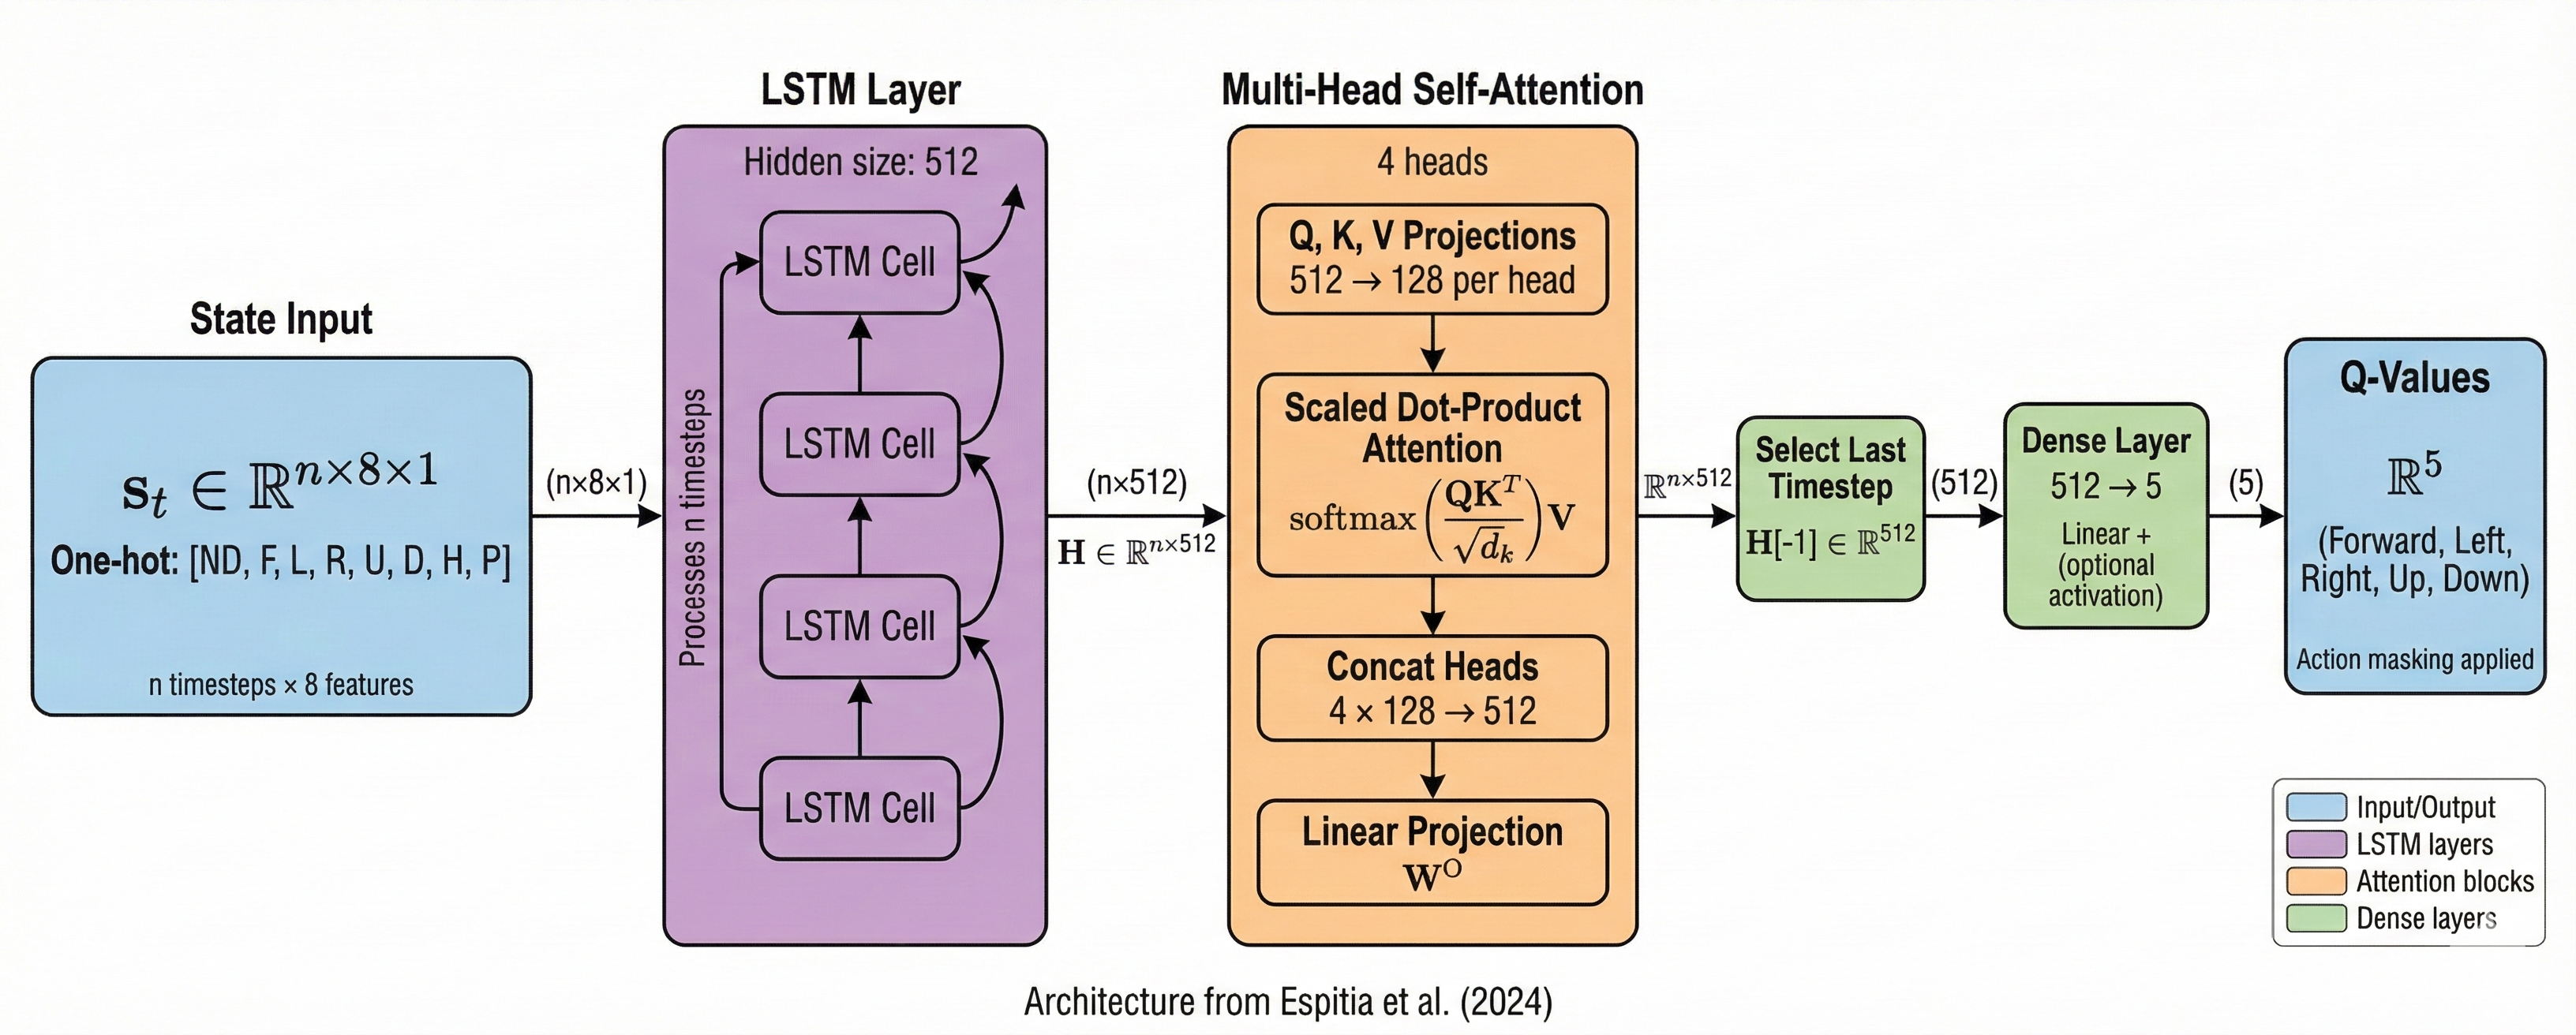
\includegraphics[width=0.95\textwidth]{fig_dqn_architecture.png}
    \caption{Attention-based Q-network used in the baseline~\cite{AttnDRL2504}. The $(n, 8, 1)$ state input is embedded and processed by a multi-head self-attention encoder, and the encoder output at the final position is mapped to Q-values for the five placement actions through a dense layer.}\label{fig:dqn_architecture}
\end{figure}

\subsubsection{Training Protocol}

The training procedure in~\cite{AttnDRL2504} uses Deep Q-Learning with several standard stabilisation techniques: a Double DQN target with a periodically synchronised target network to mitigate overestimation bias, prioritised experience replay (with annealed importance-sampling correction) so that high-TD-error transitions receive more learning signal, and an $\varepsilon$-greedy exploration policy restricted to the valid actions indicated by the environment's action mask. Full equations for these techniques follow standard formulations and are not reproduced here; we refer the reader to~\cite{AttnDRL2504} for the exact specification.

\paragraph{Hyperparameters and training details.} Following~\cite{AttnDRL2504}, separate models are trained for each benchmark sequence. Table~\ref{tab:lstm_hyperparameters} summarises the training configuration used.

\begin{table}[htbp]
\centering
\caption{Attention-based DQN training hyperparameters reported by~\cite{AttnDRL2504}.}\label{tab:lstm_hyperparameters}
\begin{tabular}{ll}
\toprule
\textbf{Parameter} & \textbf{Value} \\
\midrule
\multicolumn{2}{l}{\textit{Network Architecture}} \\
Embedding dimension $d_{\text{model}}$ & 512 \\
Attention heads & 4 \\
\midrule
\multicolumn{2}{l}{\textit{Training Configuration}} \\
Optimiser & Adam \\
Learning rate & $1.0 \times 10^{-3}$ \\
Discount factor $\gamma$ & 0.98 \\
Batch size & 16 (short seq.), 32 (long seq.) \\
Training episodes & 200K--250K (short), 500K--750K (long) \\
\midrule
\multicolumn{2}{l}{\textit{Stabilisation Techniques}} \\
Target network update & Every 1,000 steps \\
PER $\alpha$ (prioritisation) & 0.6 \\
PER $\beta$ (importance sampling) & 0.4 $\to$ 1.0 (annealed) \\
$\varepsilon$-greedy decay & $\max(0.01, 1.0 \cdot 0.9995^t)$ \\
\bottomrule
\end{tabular}
\end{table}

\section{Experiments and Results}\label{sec:results}

\subsection{Experimental Setup}

All experiments were conducted on an Apple MacBook Pro with M2 Max chip and 32 GB unified memory. The CP-SAT solver was implemented using Google OR-Tools version 9.11, while the attention-based DQN implementation was obtained from~\cite{AttnDRL2504} and executed locally. Both methods were evaluated on the standard 3D HP benchmark sequences (3d1--3d8) reported in~\cite{AttnDRL2504}, with best-known energy values serving as optimality targets.

\subsection{CP-SAT Experiments}

For CP-SAT, we allocated a total computational budget of 7 hours distributed across all 8 sequences (3d1--3d8), yielding approximately 47 minutes per sequence. Each sequence underwent a two-phase optimisation: 20\% of the budget (9 minutes, 20 seconds) for grid size exploration and parameter tuning across 5 random seeds, and 80\% of the budget (37 minutes, 20 seconds) for final optimisation with the best-discovered settings. The solver used 8 parallel worker threads throughout. All CP-SAT results reported in this chapter were obtained from our own experimental runs.

\subsection{Attention DQN Experiments}

For the attention-based DQN agent, we replicated the training protocol described in Section~\ref{sec:lstma_approach} on our local machine using the PyTorch MPS backend (M2 Max). Single-seed 200{,}000-episode runs were completed for sequences 3d1, 3d2, and 3d3; runs for 3d4 are in progress, and runs for 3d5--3d8 remain pending due to the substantial wall-clock cost of the published protocol.

We therefore report a combination of results: locally reproduced 200{,}000-episode best-evaluation energies for 3d1--3d3, with published reference values from~\cite{AttnDRL2504} used for 3d4--3d8 until local reproduction completes. Figure~\ref{fig:training_curves} shows representative training dynamics from~\cite{AttnDRL2504} for sequences of varying lengths, illustrating how training complexity scales with sequence size.

\begin{figure}[H]
    \centering    
    \begin{subfigure}[t]{0.75\textwidth}
        \centering
        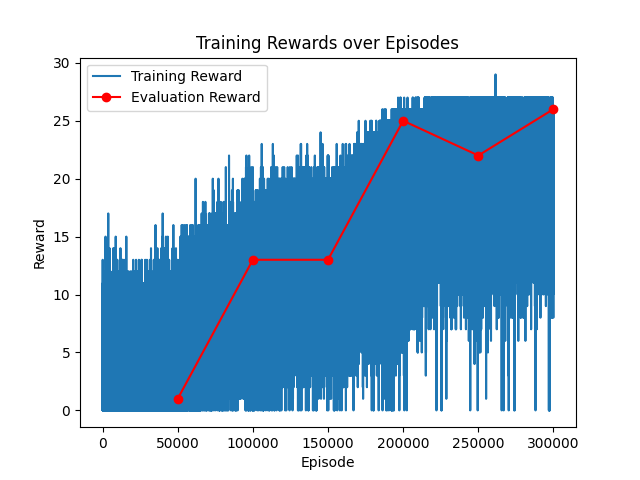
\includegraphics[width=\textwidth]{training_rewards_48.png}
        \caption{Length 48 (3d6)}\label{fig:training_48}
    \end{subfigure}
    
    % \vspace{1.5em}
    
    \begin{subfigure}[t]{0.75\textwidth}
        \centering
        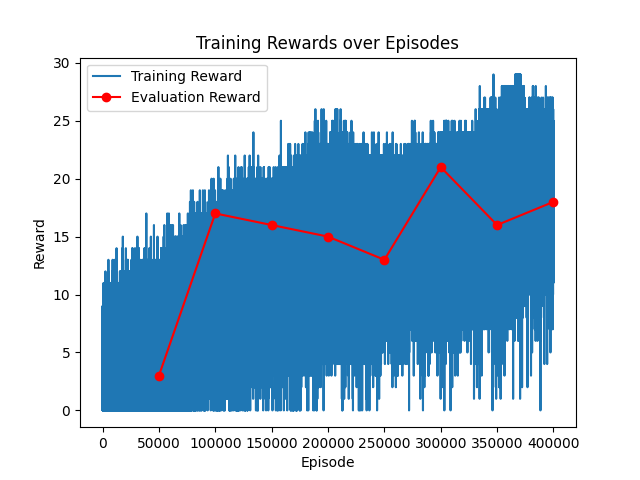
\includegraphics[width=\textwidth]{training_rewards_50.png}
        \caption{Length 50 (3d7)}\label{fig:training_50}
    \end{subfigure}
    \caption{Attention DQN training convergence curves from~\cite{AttnDRL2504} for sequences of varying lengths. Blue areas show training rewards, red lines show evaluation performance.}\label{fig:training_curves}
\end{figure}

All results tables in this chapter clearly indicate the source of each result, distinguishing between our experimental runs and values taken from the original paper.


\subsection{Solution Quality and Comparative Analysis}

Table~\ref{tab:benchmark_results} presents the energy values achieved by both methods on the 3D HP benchmark sequences. The energy is defined as the negative count of non-consecutive H-H contacts, so more negative values indicate better (more stable) conformations.

\begin{table}[htbp]
\centering
\caption{Solution quality on 3D HP benchmark sequences. Energy is the negative count of H-H contacts; lower (more negative) values are better. CP-SAT values are from this work. RL Source distinguishes locally reproduced 200{,}000-episode single-seed values (this work) from published reference values in~\cite{AttnDRL2504}.}\label{tab:benchmark_results}
\begin{tabular}{lrrrrl}
\toprule
\textbf{Seq.} & \textbf{Len} & \textbf{Best Known} & \textbf{CP-SAT} & \textbf{RL} & \textbf{RL Source}\\
\midrule
3d1 & 20 & $-11$ & $-11$ & $-10$ & local 200k \\
3d2 & 24 & $-13$ & $-13$ & $-9$  & local 200k \\
3d3 & 25 & $-9$  & $-9$  & $-9$  & local 200k \\
3d4 & 36 & $-18$ & $-18$ & $-18$ & published~\cite{AttnDRL2504} \\
3d5 & 46 & $-35$ & $-32$ & $-33$ & published~\cite{AttnDRL2504} \\
3d6 & 48 & $-31$ & $-29$ & $-30$ & published~\cite{AttnDRL2504} \\
3d7 & 50 & $-34$ & $-30$ & $-29$ & published~\cite{AttnDRL2504} \\
3d8 & 58 & $-44$ & $-40$ & $-40$ & published~\cite{AttnDRL2504} \\
\bottomrule
\end{tabular}
\end{table}

\begin{table}[htbp]
\centering
\caption{Specialised exact reference (CPSP-tools / HPstruct) on the same benchmark family. CPSP-tools enumerates a precomputed cubic-lattice H-core database offline and uses Gecode at run time to verify that the chain can be threaded around each candidate core; results are reported here as a calibration anchor for the general-purpose CP-SAT formulation rather than as a like-for-like comparison.}\label{tab:cpsp_reference}
\begin{tabular}{lrrrrl}
\toprule
\textbf{Seq.} & \textbf{Len} & \textbf{Best Known} & \textbf{CPSP/HPstruct} & \textbf{Time (s)} & \textbf{CPSP status}\\
\midrule
3d1 & 20 & $-11$ & $-11$ & 0.2 & proven optimal \\
3d2 & 24 & $-13$ & $-13$ & 0.2 & proven optimal \\
3d3 & 25 & $-9$  & $-9$  & 0.2 & proven optimal \\
3d4 & 36 & $-18$ & $-18$ & 0.2 & proven optimal \\
3d5 & 46 & $-35$ & $-35$ & 0.4 & proven optimal \\
3d6 & 48 & $-31$ & $-31$ & 0.3 & proven optimal \\
3d7 & 50 & $-34$ & $-34$ & 13.6 & proven optimal \\
3d8 & 58 & $-44$ & ---   & 1.2 & H-core DB coverage limit \\
\bottomrule
\end{tabular}
\end{table}

CPSP-tools attains the best-known energies on every sequence within its database coverage (3d1--3d7) in seconds. This is consistent with the shape of the method: the offline H-core enumeration has already pre-pruned the search to a small set of candidate cores per energy level, and the run-time work reduces to a sequence of small constraint-satisfaction queries. The CP-SAT gap on 3d5--3d7 therefore reflects the cost of a general-purpose constraint formulation that does not encode H-core structure, rather than a fundamental limit of constraint search on this benchmark family. For sequence 3d8 the bundled cubic H-core database does not contain a core large enough to accommodate the sequence's H-count; HPstruct terminates cleanly without a structure, leaving CP-SAT and the attention-DQN baseline as the only methods to report a value on this instance. The same database also cannot be reused if the lattice or model is changed, so the comparison should be read as a calibration of CP-SAT on the cubic HP family rather than as a verdict on constraint search overall.

CP-SAT matches the best-known energy values on 3d1--3d4 (lengths 20--36) and terminates with \texttt{OPTIMAL} status on these instances, providing certificates of optimality through exhaustive branch-and-bound search within the allocated time budget. The published attention DQN reference also matches best-known on 3d1--3d4. Our local 200{,}000-episode reruns of the attention DQN match best-known on 3d3 but fall short on 3d1 ($-10$ versus $-11$) and 3d2 ($-9$ versus $-13$) under a single seed and the tested budget, suggesting the reproduction settings would benefit from additional seeds or a larger compute envelope.

On longer sequences (3d5--3d8, lengths 46--58), neither method reaches the best-known values. CP-SAT maintains gaps of 2--4 contacts from the literature values and terminates with \texttt{FEASIBLE} status, unable to prove optimality within the time limit as the exponential search space growth overwhelms the constraint propagation and symmetry-breaking techniques. The published attention DQN reference shows similar performance with gaps of 2--5 contacts: $-33$ on 3d5 (within 2 of best-known), $-30$ on 3d6 (within 1), $-29$ on 3d7 (5 away), and $-40$ on 3d8. Notably, both methods converge to identical energy values on the longest sequence 3d8 (length 58), suggesting they face similar fundamental challenges in scaling to longer sequences.

Figure~\ref{fig:quality_vs_length} visualises these results, clearly showing the transition from optimal performance on shorter sequences to increasing gaps on longer ones.

\begin{figure}[H]
    \centering
    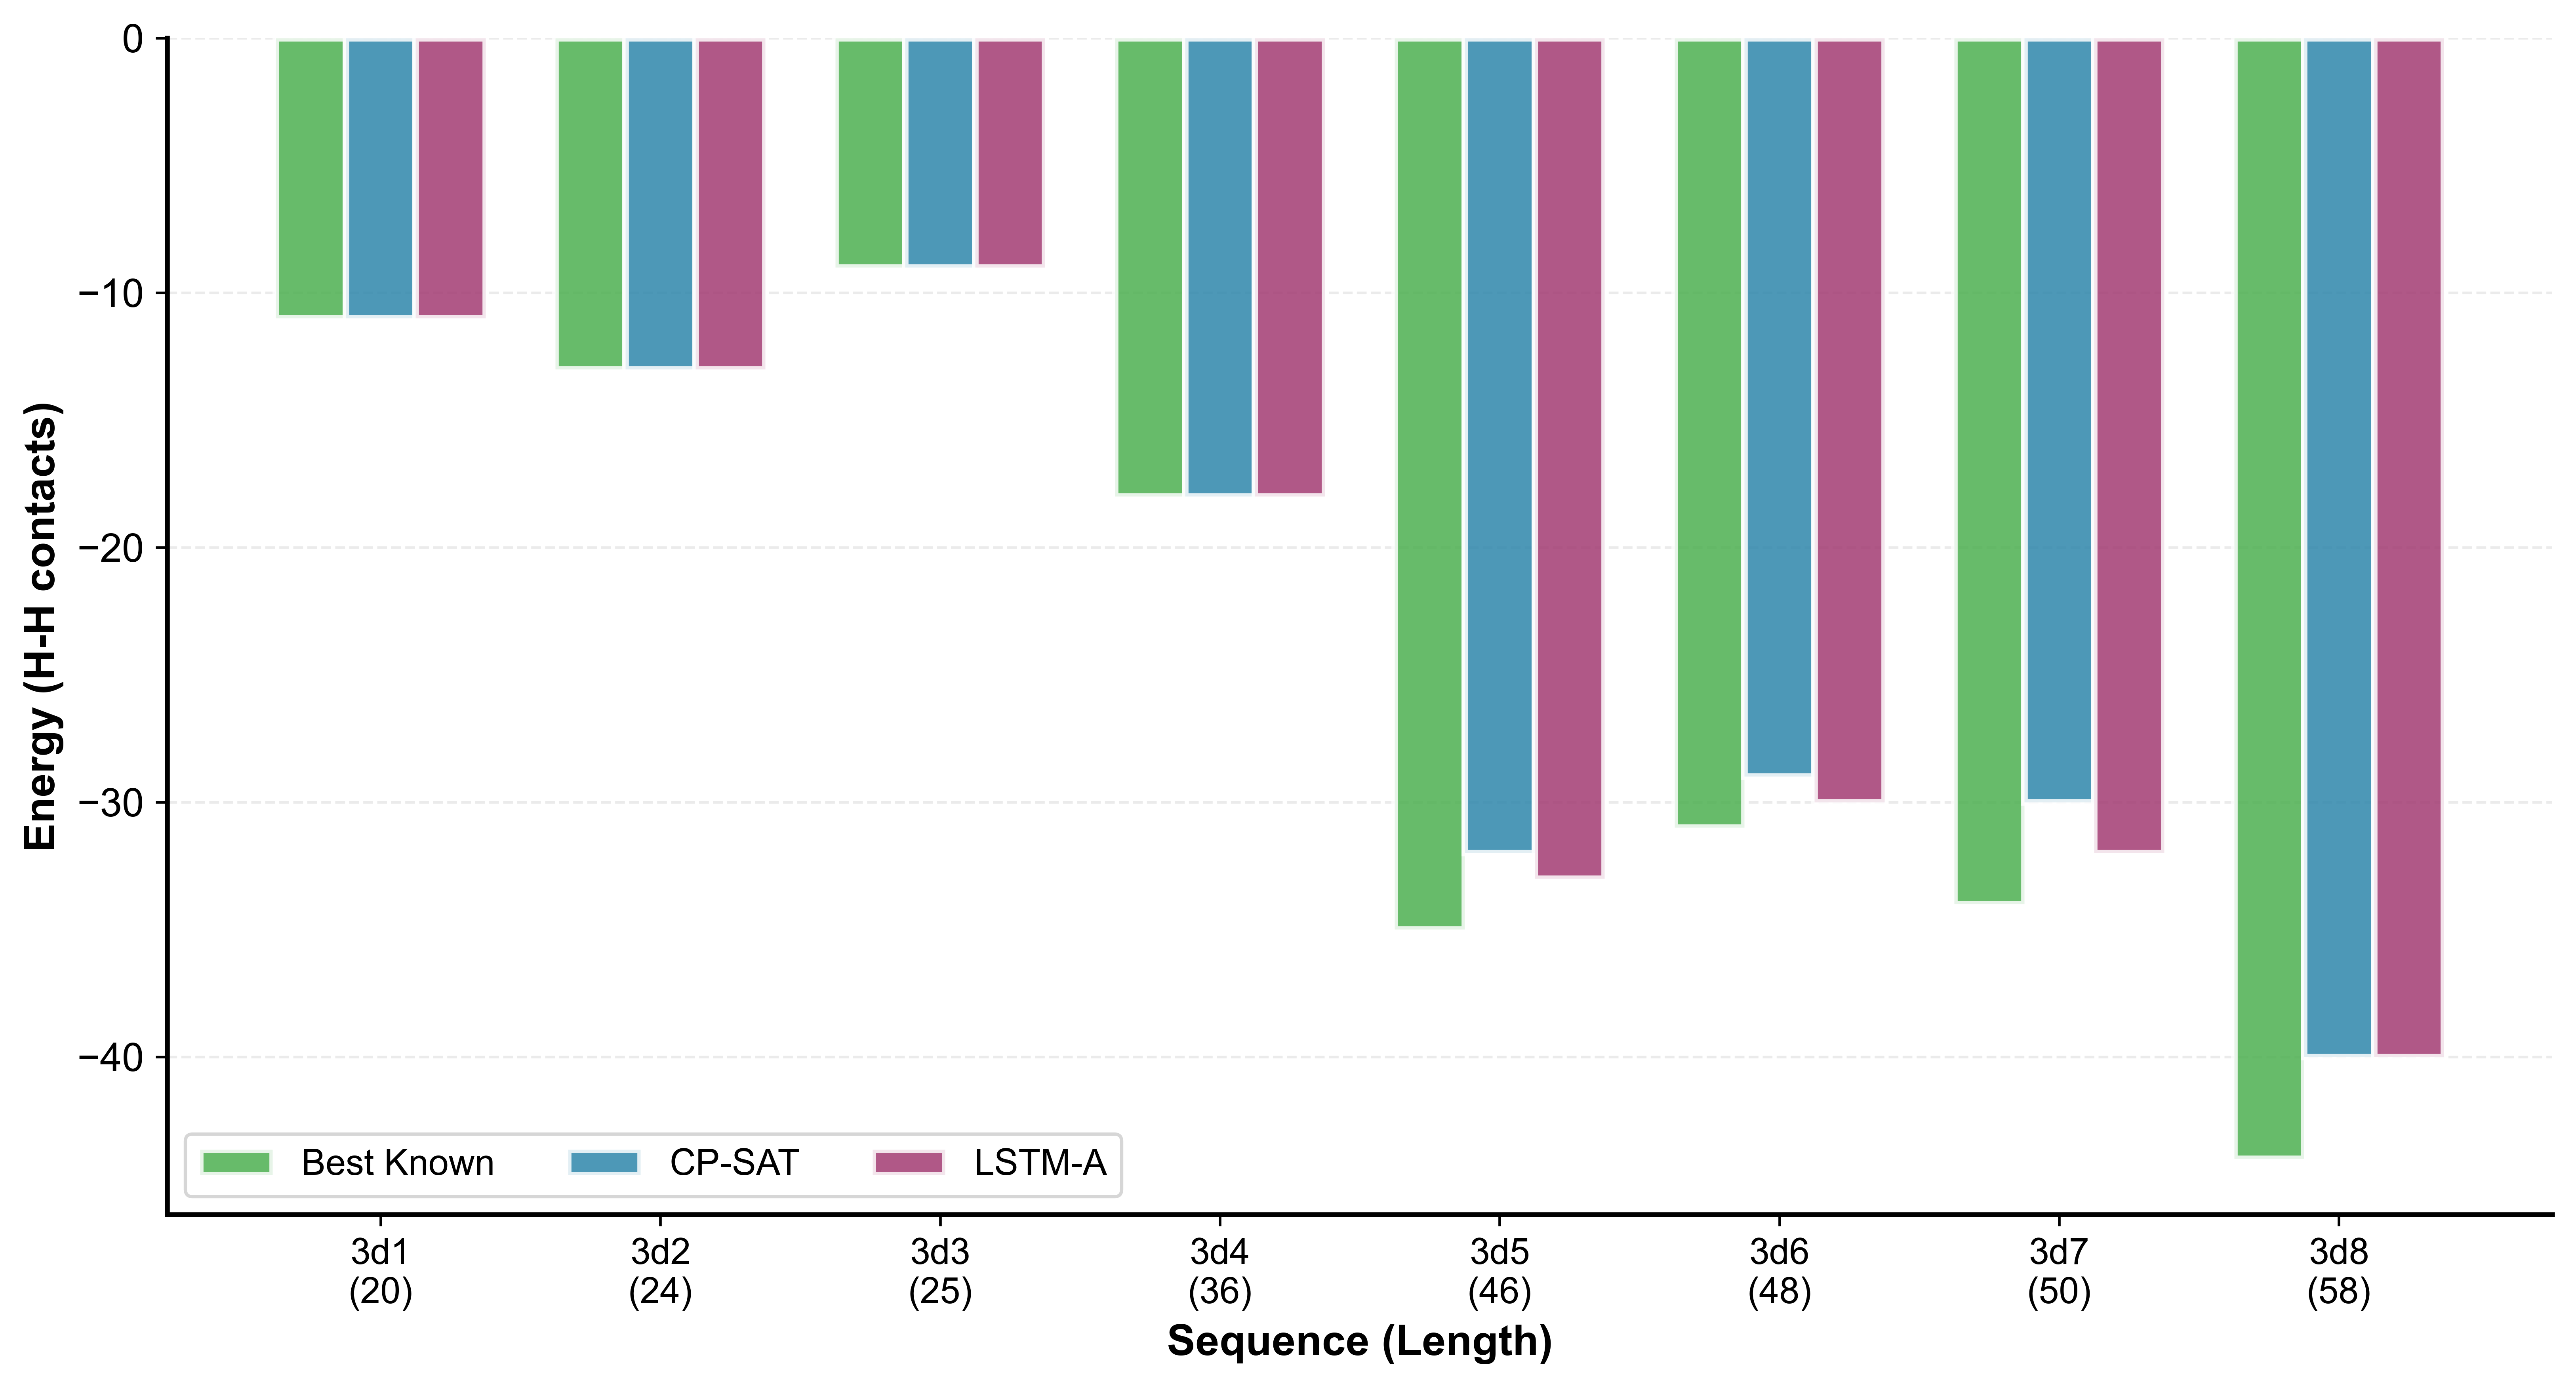
\includegraphics[width=0.9\textwidth]{fig_energy_comparison.png}
    \caption{Solution quality comparison across benchmark sequences. Both methods achieve optimal solutions for sequences up to length 36 (3d1--3d4). Performance degrades gracefully on longer sequences, with gaps of 2--5 contacts from best-known values.}\label{fig:quality_vs_length}
\end{figure}

Figure~\ref{fig:3d7_comparison} illustrates representative conformations for sequence 3d7 (length 50), where CP-SAT achieved $-30$ contacts and the published attention DQN baseline reports $-29$ contacts.

\begin{figure}[H]
    \centering
    \begin{subfigure}[t]{0.49\textwidth}
        \centering
        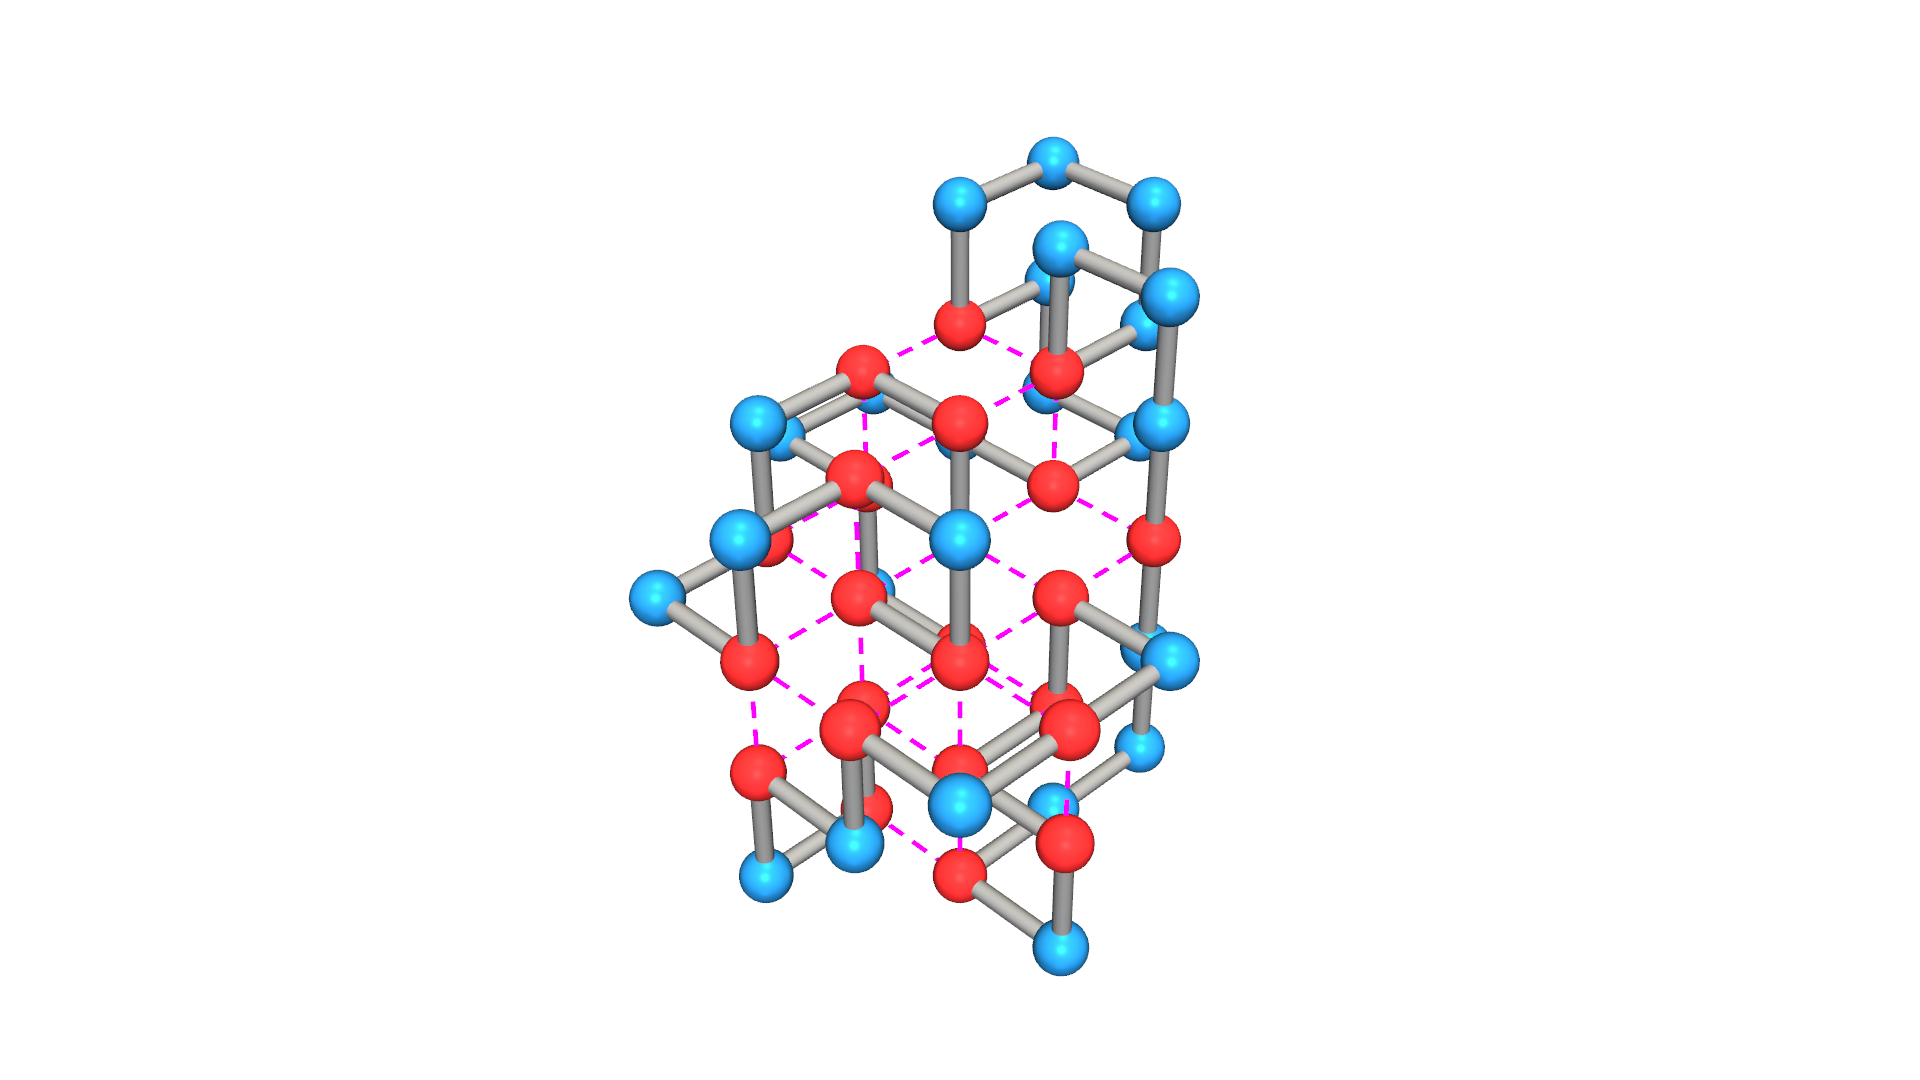
\includegraphics[width=\textwidth]{3d7_cpsat.png}
        \caption{CP-SAT solution: Energy = $-30$ contacts}\label{fig:3d7_cpsat}
    \end{subfigure}
    \hfill
    \begin{subfigure}[t]{0.49\textwidth}
        \centering
        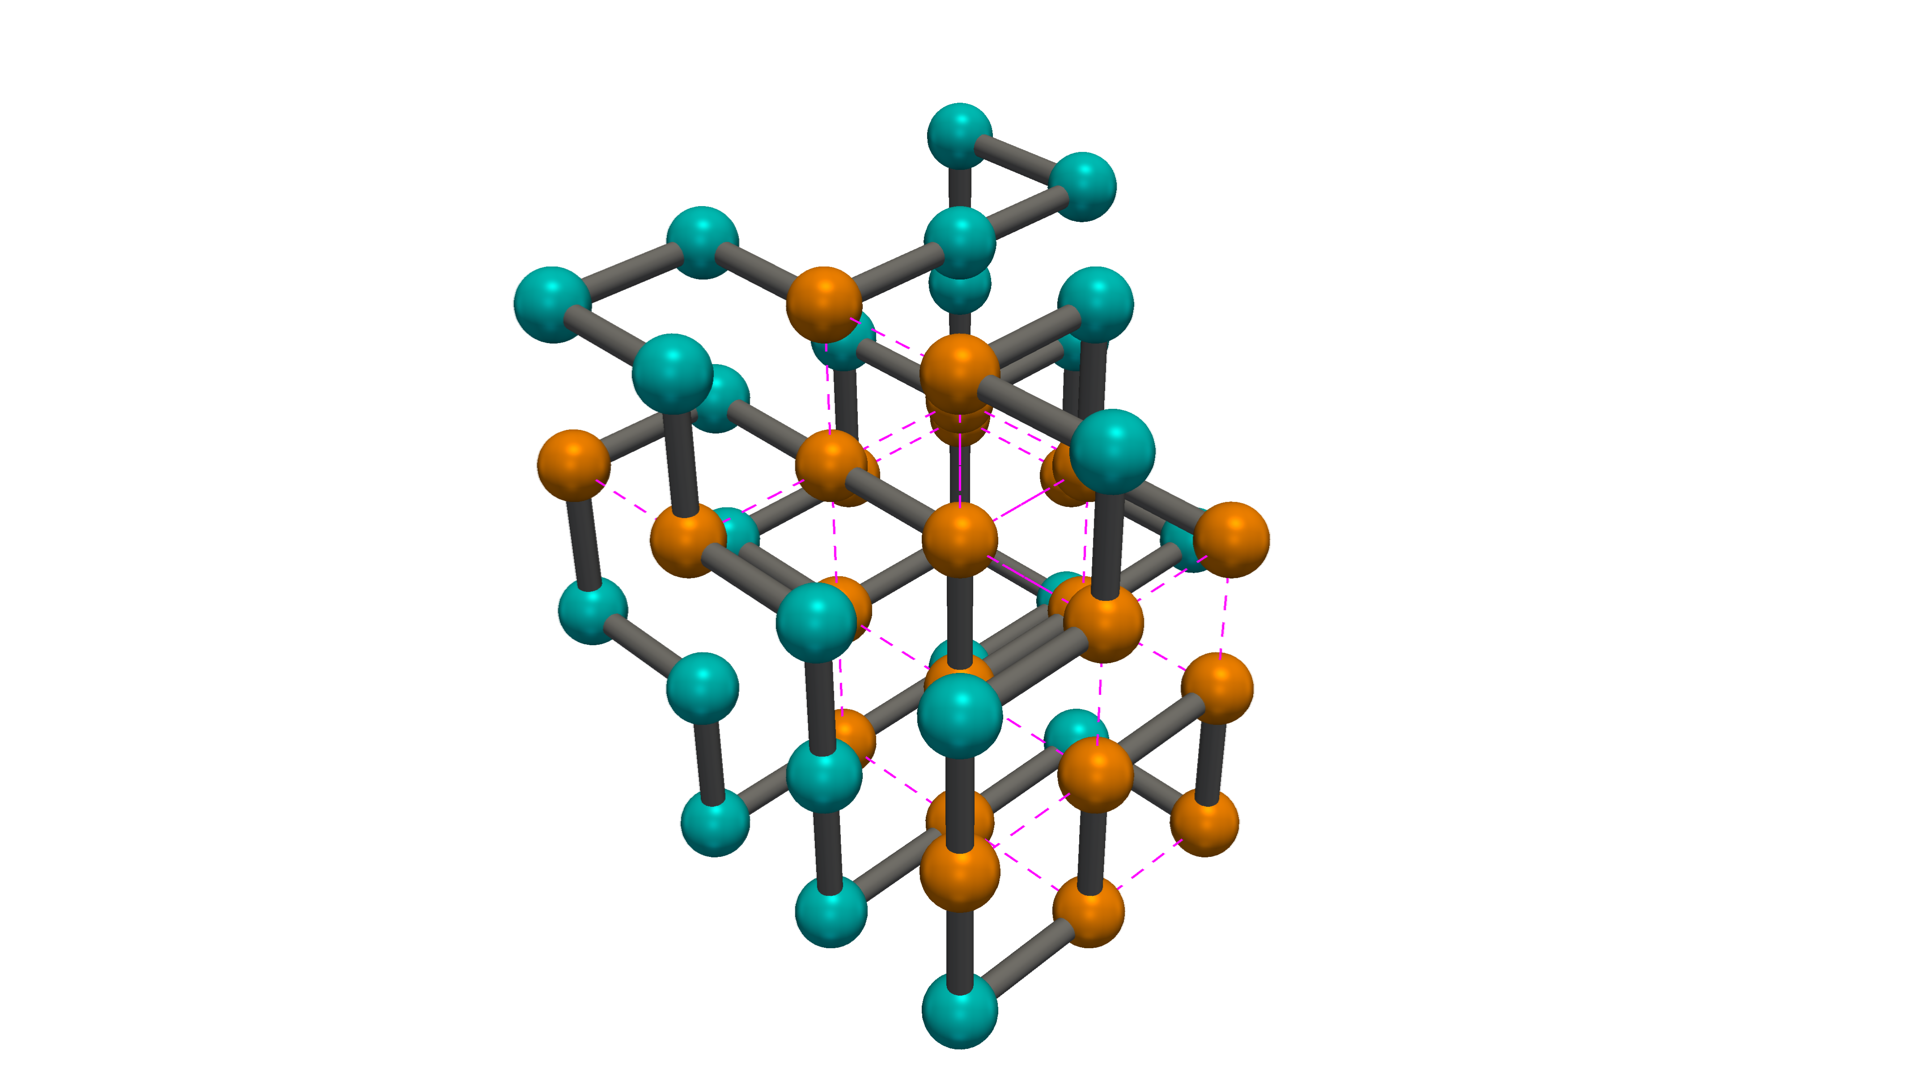
\includegraphics[width=\textwidth]{3d7_lstma.png}
        \caption{Attention DQN baseline solution: Energy = $-29$ contacts}\label{fig:3d7_lstma}
    \end{subfigure}
    \caption{Conformations for sequence 3d7 (length 50). Panel a: CP-SAT achieves $-30$ contacts (red = H, blue = P). Panel b: published attention DQN baseline achieves $-29$ contacts (orange = H, cyan = P). Magenta lines mark non-consecutive H-H contacts.}\label{fig:3d7_comparison}
\end{figure}

\section{Discussion}\label{sec:discussion}

This study compared constraint programming (CP-SAT) against an attention-based DQN reinforcement-learning baseline for the 3D HP protein folding problem, addressing whether systematic search with guarantees or learning-based exploration better handles this NP-hard combinatorial optimisation task.

On sequences up to length 36, CP-SAT and the published attention DQN baseline both reach the best-known energies, with CP-SAT additionally providing optimality certificates through exhaustive search. The attention-based architecture captures geometric patterns for maximising hydrophobic contacts, indicating that neural networks can learn useful structure of the conformational landscape. Performance diverged on longer sequences (46--58 residues), where both methods fell 2--5 contacts short of best-known values. CP-SAT's gaps reflect exponential search-space growth overwhelming constraint propagation, while the RL baseline's gaps suggest learned policies struggle to generalise beyond training distributions. Their convergence to identical energies on the longest sequence (3d8: both achieving $-40$) indicates they encounter similar local optima despite completely different search strategies.

CP-SAT provides optimality guarantees when tractable, making it ideal for benchmarking and establishing ground truth. The solver's deterministic behaviour ensures reproducibility and enables rigorous analysis through statistics. However, NP-hardness fundamentally limits scalability, and even sophisticated pruning eventually fails as the search space grows exponentially. The attention-based DQN learns placement policies from experience, potentially enabling faster solutions on similar sequences through transfer learning, and naturally models long-range relationships through self-attention.

\paragraph{Limitations.} This study has several limitations. First, CP-SAT here is a modern implementation of constraint programming for HP folding rather than a new constraint-programming theory. Second, CP-SAT wall-clock budgets and RL training episodes are not directly equivalent measures of compute, so the comparison should be interpreted as an empirical benchmark rather than a strict speed contest. Third, some RL values are taken from the published reference~\cite{AttnDRL2504} until local reproduction runs are complete; our local 200{,}000-episode single-seed reruns currently match the published reference only on 3d3 and remain below it on 3d1 and 3d2 under the tested budget, and runs for 3d4--3d8 are still in progress. Fourth, the HP model is intentionally simplified and should be viewed as a computational benchmark rather than a realistic all-atom protein-folding model. Fifth, CPSP-tools is not an apples-to-apples baseline for CP-SAT. Its solution speed reflects an offline H-core precomputation, and it returns no result for sequences whose H-count exceeds the bundled database (as observed on 3d8) or for lattice variants other than 3D cubic.

Future work should explore hybrid approaches combining CP-SAT's optimality-seeking with the RL baseline's pattern recognition, for example using CP-SAT to generate diverse training data or using learned policies to warm-start branch-and-bound search. Transfer learning also deserves investigation: can models pretrained on shorter sequences accelerate longer ones, and do they transfer across sequences with similar hydrophobic patterns? Hybrid pipelines that warm-start CP-SAT with H-core skeletons drawn from CPSP-tools, or that use CP-SAT to extend coverage beyond the precomputed H-core database (as required for sequences such as 3d8 and for non-cubic lattices), are a natural next step.

\section*{Code Availability}

The software, code, and data used in this study are available in public GitHub repositories and Github Gists:

\begin{itemize}
    \raggedright%
    \item \textbf{CP-SAT Implementation:}\\
    \url{https://github.com/pranav-ramanathan/HP-CSP}
    \item \textbf{Attention-based DQN Baseline Implementation:}\\
    \url{https://github.com/AnonymousAuthor117/Protein-Structure-Prediction-in-the-3D-HP-Model-Using-Deep-Reinforcement-Learning}
    % [TODO-DATA: replace URL with the official repository associated with arXiv:2504.15634 once located]
    \item \textbf{CPSP-tools reference runs:}\\
    \texttt{scripts/run\_cpsp\_reference.py}, \texttt{scripts/analyze\_cpsp\_reference.py}, \texttt{results/cpsp\_reference/}
    \item \textbf{Image Generation Prompts:}\\
    \url{https://gist.github.com/pranav-ramanathan/f5a4f8effa07861ef452e802132e2dc8}
\end{itemize}


\bibliographystyle{unsrtnat}
\bibliography{references}

\end{document}
